% 第8章：黑洞理论
\section{黑洞理论}
\label{sec:bh}

\subsection{经典GR中的奇点问题}

广义相对论预言了奇点的存在——时空曲率和物质密度发散的点。史瓦西解表明当 $r \to 0$ 时：
\begin{equation}
    g_{tt} \to -\infty, \quad g_{rr} \to \infty, \quad \rho \to \infty
\end{equation}

这表明广义相对论在黑洞中心失效。

奇点导致三个主要悖论：
\begin{enumerate}
    \item \textbf{物理奇点}：无限密度是非物理的
    \item \textbf{信息悖论}：霍金辐射表现为热的，暗示信息丢失
    \item \textbf{防火墙悖论}：量子纠缠的要求似乎违反等效原理
\end{enumerate}

我们的框架通过分形-扭转模型解决了所有三个问题。

\subsection{分形-扭转黑洞模型}

\subsubsection{核心假设}

\begin{hypothesis}[扭转饱和核心]
黑洞中心不是奇点，而是一个\textbf{扭转饱和的分形核心}，其中：
\begin{enumerate}
    \item 时空具有谱维 $d_s < 4$ 的分形结构
    \item 扭转达到最大临界值 $\tau_{max}$
    \item 核心具有有限密度和规则几何
\end{enumerate}
\end{hypothesis}

\begin{figure}[htbp]
\centering
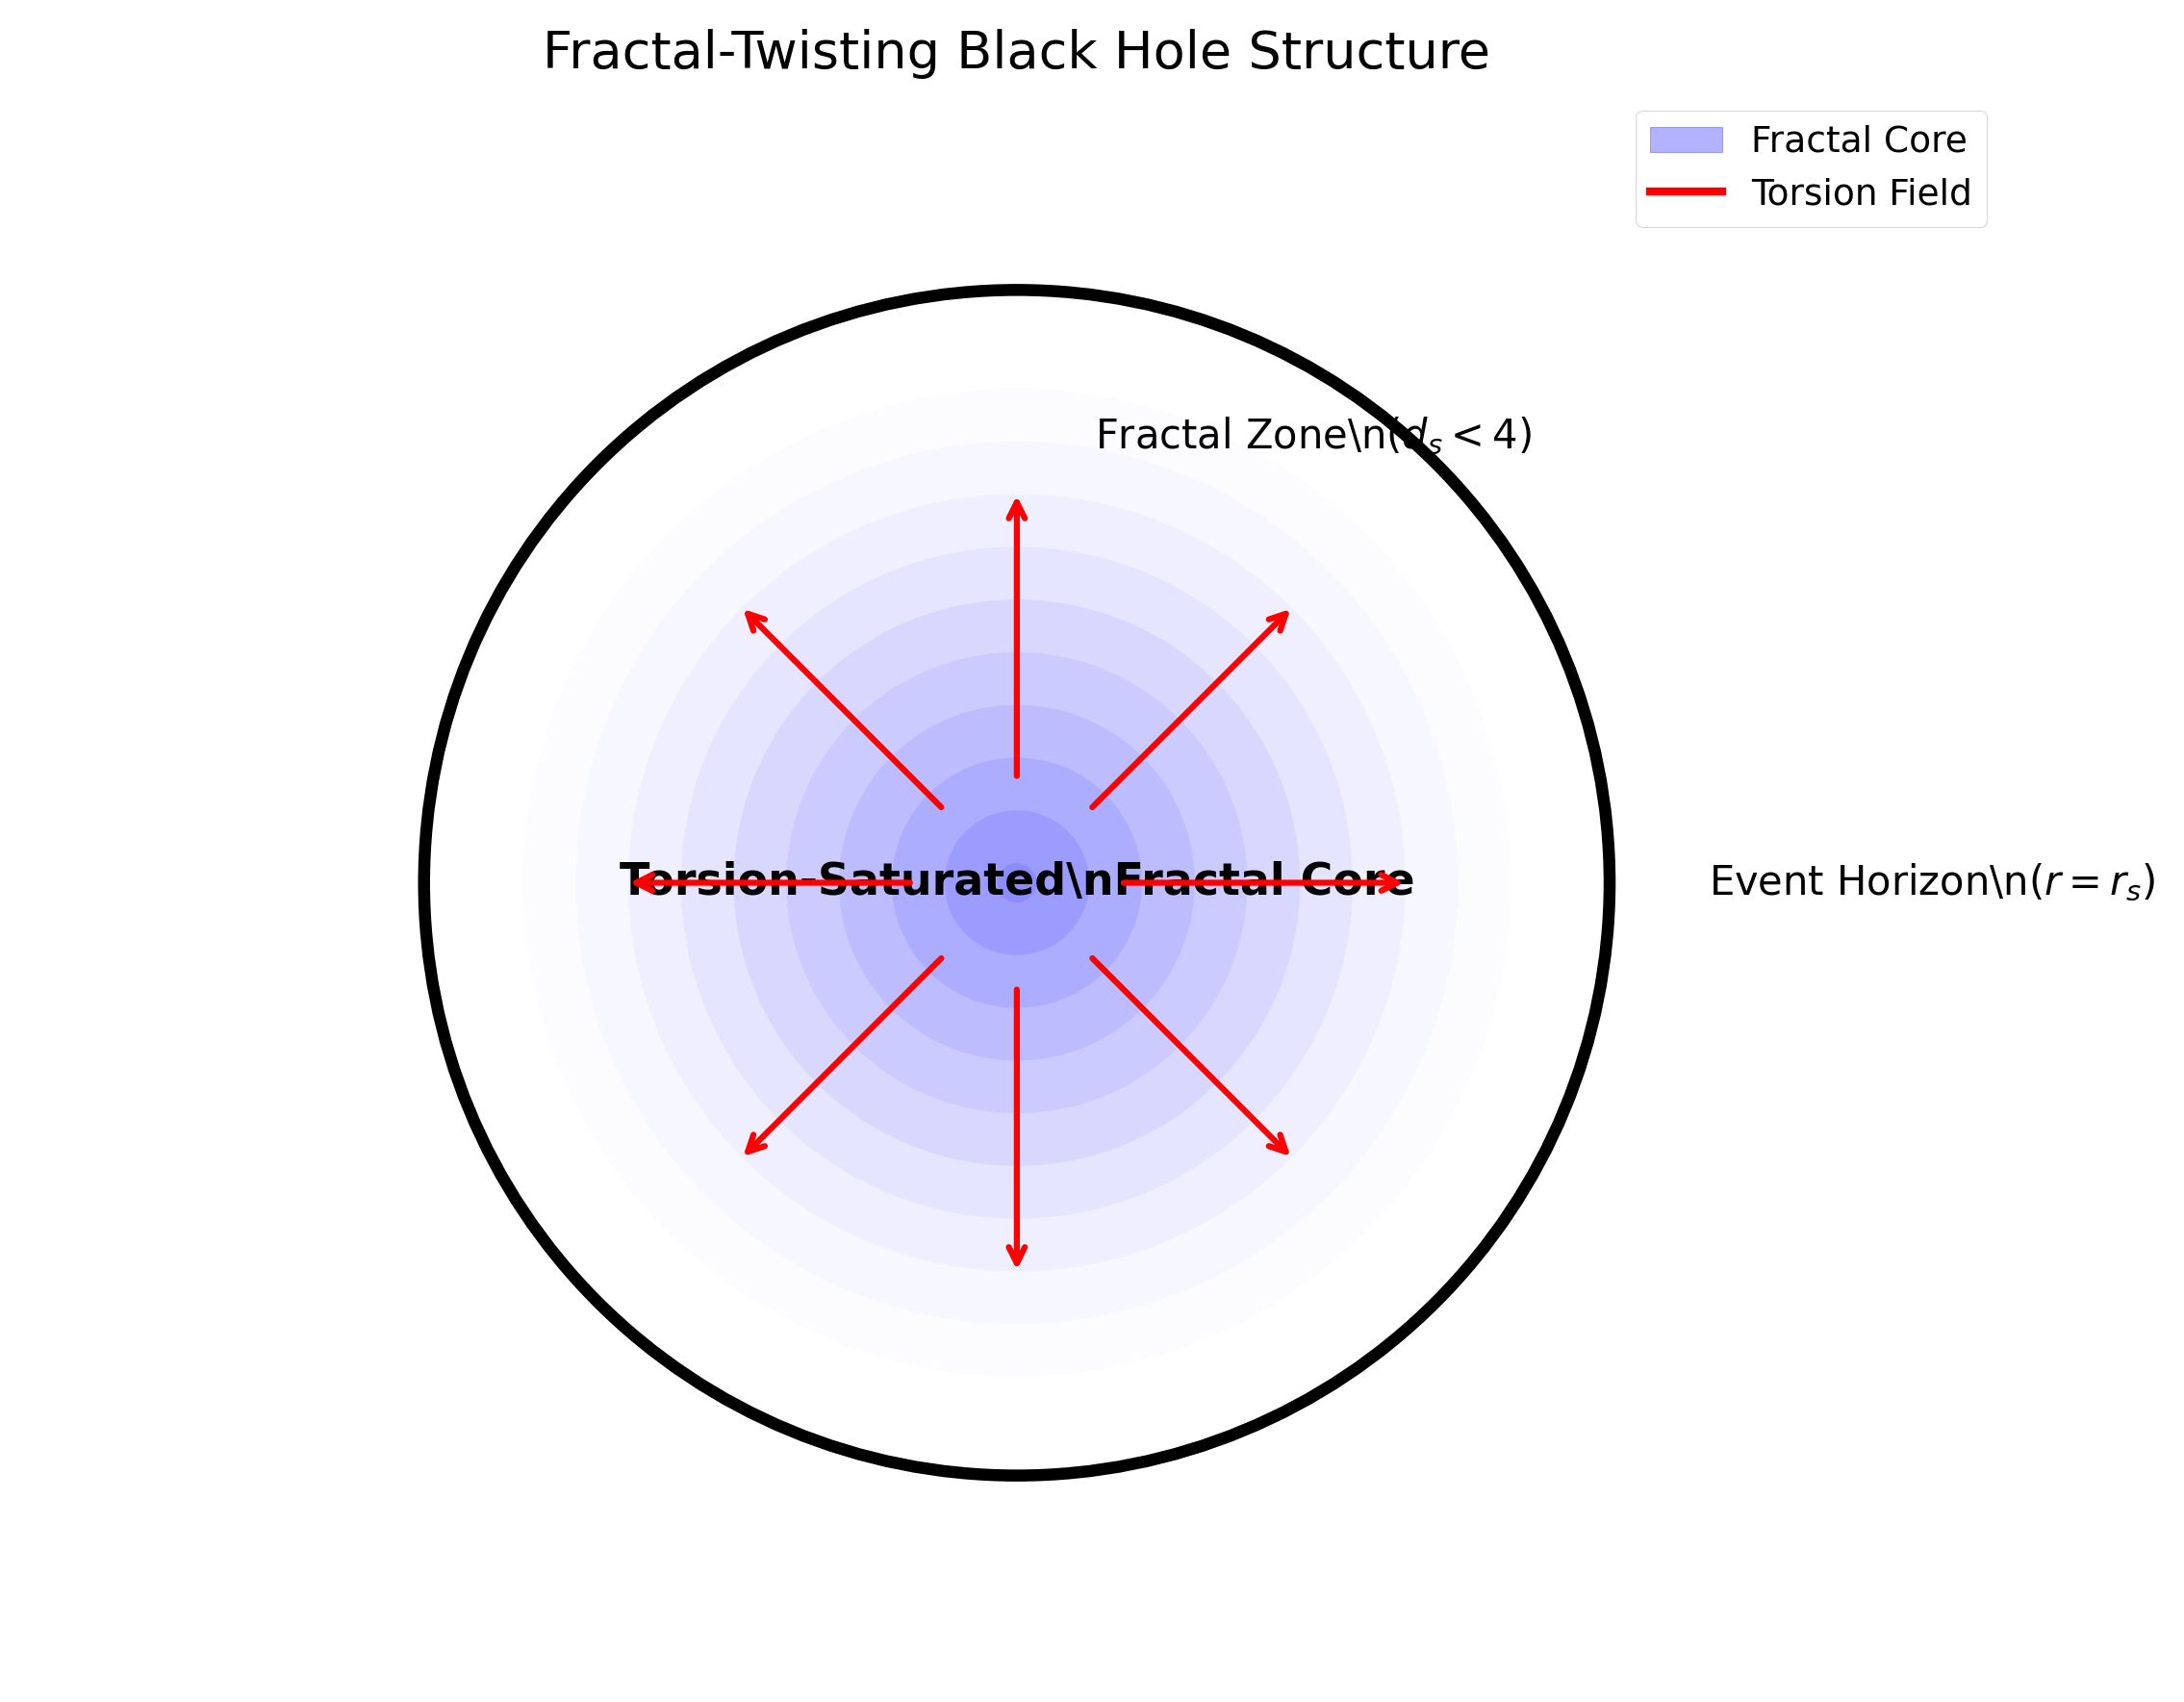
\includegraphics[width=0.7\textwidth]{figures/fig4_black_hole.png}
\caption{分形-扭转黑洞结构。中心区域包含一个扭转饱和的分形核心（蓝色），$d_s < 4$，被事件视界包围。扭转场线（红色箭头）从核心径向向外。}
\label{fig:black_hole}
\end{figure}

\subsubsection{形成机制}

形成通过四个阶段进行：

\textbf{阶段1：引力坍缩}
物质在引力作用下坍缩，密度增加：
\begin{equation}
    \rho(r) = \frac{M}{\frac{4}{3}\pi r^3}
\end{equation}

\textbf{阶段2：扭转增强}
能量-动量张量产生时空扭转：
\begin{equation}
    \tau_{\mu\nu} \propto T_{\mu\nu}
\end{equation}

\textbf{阶段3：扭转饱和}
当 $\tau \to \tau_{crit}$，扭转饱和：
\begin{equation}
    \tau_{max} = \frac{c^3}{G\sqrt{\rho_{Planck}}}
\end{equation}

\textbf{阶段4：分形核心形成}
中心区域形成具有自相似性的有限密度、扭转饱和分形结构：
\begin{equation}
    d_H = 2 + \frac{\alpha}{2GM/rc^2}
\end{equation}

\subsubsection{奇点消除}

\begin{theorem}[规则核心定理]
在分形-扭转模型中，当 $r \to 0$ 时总应力-能量张量保持有限：
\begin{equation}
    T^{total}_{\mu\nu} = T^{(matter)}_{\mu\nu} + T^{(torsion)}_{\mu\nu} < \infty
\end{equation}
其中 $T^{(torsion)}_{\mu\nu} = -\alpha(\tau^2 + \frac{1}{3}\tau^4)g_{\mu\nu}$ 提供抵消物质发散的负压。
\end{theorem}

最大密度为：
\begin{equation}
    \rho_{max} = \frac{c^6}{G^3M^2}
\end{equation}

对于恒星质量黑洞（$M \sim 10M_\odot$）：
\begin{equation}
    \rho_{max} \sim 10^{76} \text{ kg/m}^3
\end{equation}

虽然极高，但这是有限的，远低于普朗克密度。

\subsection{信息悖论的解决}

\subsubsection{扭转模式中的信息编码}

落入黑洞的信息不会丢失，而是以分形核心的量子化扭转模式编码：

\begin{equation}
    |\psi_{in}\rangle \to |\psi_{twist}\rangle = \sum_n c_n |n\rangle_{twist}
\end{equation}

其中 $|n\rangle_{twist}$ 是扭转场的本征态。

\subsubsection{重新审视霍金辐射}

霍金温度被扭转效应修正：
\begin{equation}
    T_H = \frac{\hbar c^3}{8\pi GMk_B}(1 + \beta\tau_0^2)
\end{equation}

其中 $\beta$ 是依赖于黑洞质量的数值因子。

更重要的是，辐射不是纯粹热的，而是携带关于扭转模式的信息：
\begin{equation}
    \rho_{rad} = \rho_{thermal} + \rho_{info}
\end{equation}

\subsubsection{信息守恒}

\begin{theorem}[信息守恒]
包括黑洞和辐射的总量子态演化保持纯态：
\begin{equation}
    S_{total} = S_{BH} + S_{rad} + S_{corr} = 0
\end{equation}
其中 $S_{corr}$ 代表黑洞内部与发射辐射之间的关联。
\end{theorem}

当黑洞蒸发时，信息通过霍金辐射中的微妙关联逐渐释放。

\subsection{量子黑洞遗迹}

\subsubsection{遗迹的形成}

当黑洞蒸发到普朗克尺度时，由于扭转饱和，蒸发停止：

\begin{equation}
    M_{remnant} \sim M_{Planck} \cdot \tau_0^{1/3} \sim 10^{-8} \text{ kg}
\end{equation}

\subsubsection{遗迹的性质}

\begin{itemize}
    \item \textbf{质量}：$M_{rem} \sim 10^{-8}$ kg
    \item \textbf{大小}：$R_{rem} \sim 10^{-35}$ m（普朗克尺度）
    \item \textbf{温度}：$T_{rem} \sim 10^{32}$ K
    \item \textbf{寿命}：稳定（蒸发停止）
\end{itemize}

\subsubsection{与暗物质的联系}

\begin{proposition}[作为暗物质的遗迹]
在早期宇宙中形成并已蒸发为遗迹的 today 原初黑洞可能构成暗物质的显著部分。
\end{proposition}

丰度估计为：
\begin{equation}
    \Omega_{rem} \sim 10^{-8} \cdot f_{PBH} \cdot \Omega_{DM}
\end{equation}

其中 $f_{PBH}$ 是原初黑洞在暗物质中的比例。

\subsection{黑洞熵}

Bekenstein-Hawking熵接收来自分形结构的修正：

\begin{equation}
    S_{BH} = \frac{A}{4G\hbar}(1 + \gamma \tau_0^2 \ln(A/A_{Planck}))
\end{equation}

其中 $A$ 是视界面积，$\gamma$ 是无量纲常数。

这可以解释为计数扭转模式的微观状态：
\begin{equation}
    S_{BH} = k_B \ln \mathcal{N}_{twisting} \sim k_B \frac{A}{\ell_P^2}
\end{equation}

\subsection{观测信号}

\subsubsection{合并引力波}

分形核心修正了振铃信号：
\begin{equation}
    h(t) = h_0 e^{-t/\tau_{QNM}} \cos(\omega_{QNM}t)(1 + \delta h_{twist})
\end{equation}

其中 $\delta h_{twist}$ 是扭转依赖的修正。

\subsubsection{阴影成像}

事件视界望远镜可以检测与克尔阴影的偏差：
\begin{equation}
    \delta \theta_{shadow} \sim \tau_0^2 \cdot \theta_{Kerr} \sim 10^{-12} \text{ radians}
\end{equation}

当前分辨率不足，但未来仪器可能达到灵敏度。

\subsubsection{暗物质探测}

量子遗迹可以通过以下方式探测：
\begin{itemize}
    \item 具有特征光曲线的微引力透镜事件
    \item 中子星的异常加热
    \item 引力波信号
\end{itemize}

\subsection{总结}

分形-扭转黑洞模型解决了：
\begin{enumerate}
    \item \textbf{奇点问题}：被有限密度扭转饱和核心取代
    \item \textbf{信息悖论}：信息保存在扭转模式中
    \item \textbf{防火墙悖论}：视界处没有高能辐射
\end{enumerate}

此外，该模型预测：
\begin{itemize}
    \item 作为暗物质候选者的量子遗迹
    \item 具有信息内容的修正霍金辐射
    \item 引力波和阴影成像中的可观测信号
\end{itemize}

这完成了统一场论框架内黑洞的一致描述。
